\documentclass{article}

%Packages
\usepackage{amsmath}
\usepackage{amsfonts}
\usepackage{amssymb}
\usepackage{tikz}
	\usetikzlibrary {arrows.meta} 
	\usetikzlibrary{calc}
\usepackage{polski}
\usepackage{array} % Required for tables
\usepackage{animate}
\usepackage{hyperref}
\usepackage{hyperref}
\usepackage[left=2cm, top=2cm, right=2cm, bottom=1cm, includeheadfoot, headheight=50pt, a4paper]{geometry}
\title{Tandetna seria tekstów matemetycznych}
\author{Ciekawe rzeczy o średnich}
\newcommand{\abs}[1]{\left|#1\right|}
\newcommand{\rad}{\text{rad}}
\usepackage{graphicx} % Required for inserting images
\graphicspath{ {./img} }

\begin{document}
\maketitle
\section{Wstęp}
Działa czy nie działa??? Ala pije po 2 piwa w soboty i niedziele a Bob --- 1 piwo w patrzyste dni i pół w nieparzyste. Kto pije więcej?\\
\textbf{Rozwiązanie.} Ala pije średnio $\frac{0+0+0+0+0+2+2}7=\frac47$ piwa dziennie a Bob --- $\frac{1+0.5}2=\frac34$. Oczywiście $\frac34>\frac47$ więc Bob pije więcej.\\
Ten przykład pokazuje do czego można użyć średnich w prawdziwym życiu. Teraz do rzeczy:
\section{Średnia}
To słowo bez kontekstu oznacza średnią arytmetyczną, czyli\[\bar a = \frac{a_1+a_2+\cdots+a_n}n\]albo $\frac1n\sum a_i$. Elementy ciągu $a$ nazywamy \textit{danymi}.
Ewentualnie jeśli nie chodzi nam o ciąg tylko o całą funkcję o dziedzinie $(0, \Delta x)$:
\[\bar f = \lim_{n\to\infty}\frac1n\sum_{i=0}^{n} f(x_i) = \frac1{\Delta x}\int_0^{\Delta x}f(x)dx = \frac{\Delta F}{\Delta x}\]
dla $x_i=\frac in\cdot\Delta x$ i $F'(x)=f(x)$.
Przedział $(0, \Delta x)$ można zastąpić przez $(a, b)$ ale wtedy wzory będą brzydsze. 
Zwykle nazywa się to wartością średnią funkcji $f(x)$, np jeśli przyjmiemy taką zmianę oznaczeń:
\begin{align*}
	\text{współrzędna } x &\to \text{czas }t\\
	\text{funkcja }f(x) &\to \text{prędkość }v(t)\\
	\text{funkcja }F(x)\text{ której pochodną jest }F'(x)=f(x) &\to \text{droga }s(t)\text{ której pochodną jest }s'(t)=v(t)\\
	\bar f = \frac1{\Delta x}\int_0^{\Delta x}f(x)dx = \frac{\Delta F}{\Delta x} &\to v_\text{śr} = \frac1{\Delta t}\int_0^{\Delta t}v(t)dt = \frac{\Delta s}{\Delta t}
\end{align*}
…to będziemy ją nazywać średnią wartością prędkości albo prędkością średnią.
Tak samo działa to dla średniego ciśnienia ($\frac{\Delta F}{\Delta S}$), natężenia prądu ($\frac{\Delta q}{\Delta t}$), gęstości ($\frac{\Delta m}{\Delta V}$) itd.\\
Dalej będziemy oznaczać średnie funkcji przez $\bar a$, a średnie danych $a_1, a_2, \cdots, a_n$ przez $\mu(a_1, a_2, \cdots, a_n)$
\subsection{Średnia ważona}
Kiedy chcemy żeby ta sama dana trafiła do średniej ileś razy, tak jak trójka przy $\frac{3+3+3+3+2+2+5}{7}$ to przypisujemy jej wagę, w tym wypadku 4 bo są 4 trójki.
Ogólnie wzór na średnią ważoną wygląda tak:
\[\bar a = \frac{\sum w_ia_i}{\sum w_i}\]
Gdzie $w_i$ jest wagą danej $a_i$, która domyślnie wynosi 1.
\subsection{Łączenie średnich}
jeśli weźmiemy ciąg $(a_1, a_2, \cdots)$, po czym podzielimy go na $n$ podciągów równej długości $(a_1, \cdots, a_n), (a_{n+1}, \cdots, a_{2n}), \cdots$
o średnich odpowiednio $s_1, s_2, \cdots$, to wartość średnia całego ciągu wynosi\[
	\bar a =\frac{s_1+s_2+\cdots}{n}
\]
Jeżeli ich długości nie będą takie same, tylko $i$-ty podciąg będzie miał długość $\ell_i$, to\[
	\bar a =\frac{\ell_1s_1+\ell_2s_2+\cdots}{\ell_1+\ell_2+\cdots}
\]
Jeżeli dodatkowo dodamy wagi, a suma wag w $i$-tym podciąg będzie miał wynosić $W_i$, to\[
	\bar a =\frac{W_1s_1+W_2s_2+\cdots}{W_1+W_2+\cdots}
\]
W skrócie chodzi o to, że średnia średnich jest średnią, tak samo jak suma sum jest sumą. W ten sposób można definiować średnie dla rzeczy których nie da się zsumować.
\subsection{Uśrednianie punktów}
Średnia punktów $A$ i $B$ to środek odcinka $AB$. Za to ich średnia ważona o wagach $w_A$ i $w_B$ to taki punkt $M$ na tym odcinku że sotsunek jego odległości od każdego z końców jest taki sam jak stosunek wag, tj.\[
	\frac{MB}{MA}=\frac{w_A}{w_B}
\]Obrazek:
\begin{center}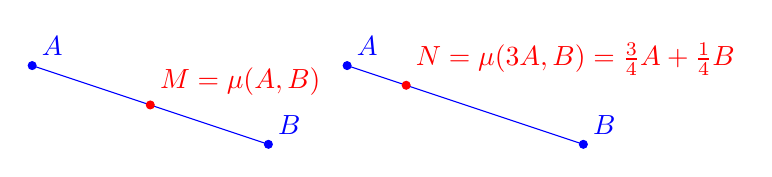
\begin{tikzpicture}
	\filldraw[blue] (0, 0) circle (0.05) node[above right] {$A$};
	\filldraw[blue] (3, -1) circle (0.05) node[above right] {$B$};
	\draw[blue] (0, 0) -- (3, -1);
	\filldraw[red] (1.5, -.5) circle (0.05) node[above right] {$M=\mu(A, B)$};

	\filldraw[blue] (4, 0) circle (0.05) node[above right] {$A$};
	\filldraw[blue] (7, -1) circle (0.05) node[above right] {$B$};
	\draw[blue] (4, 0) -- (7, -1);
	\filldraw[red] (4.75, -.25) circle (0.05) node[above right] {$N=\mu(3A, B)=\frac34A+\frac14B$};
\end{tikzpicture}\end{center}
Jeśli stosunek $\frac{w_A}{w_B}$ jest wymierny, to można równie dobrze korzystać ze wzorów na nie-ważoną średnią i łączenie średnich, np $N$ można policzyć jako $\mu(A, M)$.
Oczywiście, to samo wyszłoby gdybyśmy uśrednili współrzędne punktów (tzn. współrzędna $x$ punktu $m$ to śrenia współrzędnych $x$ punktów $A$ i $B$), o ile mamy jakiś układ współrzędnych.\\
Czasami średnią 2 punktów nazywa się (uwaga długie słowo) interpolacją liniową (LERP-em od \textit{linear interpolation}); wtedy zamiast wag podaje się ile \% ich sumy zajmuje 1 z nich.\\
Za to średnią 3 punktów liczymy tak:
\\\textbf{Twierdzenie 1. Odcinki łączące środki boków trójkąta z wierzchołkami naprzeciwko nich przecinają się w 1 punkcie, który:
\\\indent 1) istnieje, 
\\\indent 2) dzieli każdy z nich w stosunku 1:2, 
\\\indent 3) jest średnią wierzchołków trójkąta (barycentrum).
\\Dowód. }Oznaczmy wierzchołki $A$, $B$, i $C$ w dowolnej kolejności.
Śrenia wierzchołków $A$ i $B$ to środek odcnika $AB$ (dalej $M$), a średnia wszystkich wierzchołków ($G$) to średnia $M$ z wagą 2 i $C$ z wagą 1, tj.\[
	G=\frac{2M+C}{3}
\]A więc leży na odcinku $MC$, 2 razy bliżej do $M$ niż do $C$.
Ponieważ wierzchołki oznaczyliśmy dowolnie a punkt $G$ jest tylko 1, to odcinki z $MC$ i spółka przecinają się w 1 punkcie $\square$.
\begin{center}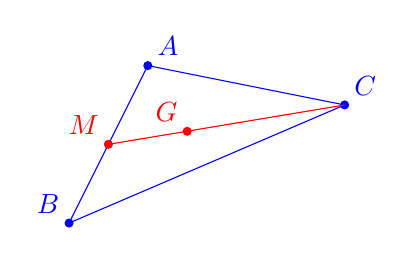
\begin{tikzpicture}
	\filldraw[blue] (0, 0) circle (0.05) node[above right] {$A$};
	\filldraw[blue] (-1, -2) circle (0.05) node[above left] {$B$};
	\filldraw[blue] (2.5, -.5) circle (0.05) node[above right] {$C$};
	\draw[blue] (0, 0) -- (-1, -2);
	\draw[blue] (-1, -2) -- (2.5, -.5);
	\draw[blue] (2.5, -.5) -- (0, 0);

	\filldraw[red] (-.5, -1) circle (0.05) node[above left] {$M$};
	\draw[red] (-.5, -1) -- (2.5, -.5);

	\filldraw[red] (.5, -.835) circle (0.05) node[above left] {$G$};
\end{tikzpicture}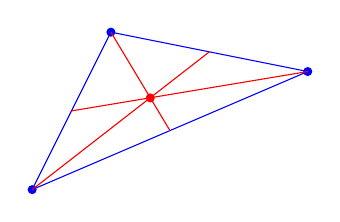
\begin{tikzpicture}
	\filldraw[blue] (0, 0) circle (0.05);% node[above right] {$A$};
	\filldraw[blue] (-1, -2) circle (0.05);% node[above left] {$B$};
	\filldraw[blue] (2.5, -.5) circle (0.05);% node[above right] {$C$};
	\draw[blue] (0, 0) -- (-1, -2);
	\draw[blue] (-1, -2) -- (2.5, -.5);
	\draw[blue] (2.5, -.5) -- (0, 0);

	%\filldraw[red] (-.5, -1) circle (0.05);% node[above left] {$M$};
	\draw[red] (-.5, -1) -- (2.5, -.5);
	\draw[red] (1.25, -.25) -- (-1, -2);
	\draw[red] (.75, -1.25) -- (0, 0);

	\filldraw[red] (.5, -.835) circle (0.05);% node[above left] {$G$};
\end{tikzpicture}\end{center}
Podobnie to liczymy dla $n$ punktów; tutaj ciekawym faktem jest że ich średnia zawsze będzie we wnętrzu ich otoczki wypukłej, tzn figury o najmniejszym obwodzie która je zawiera.
Dowód jest łatwy przez indukcję.
Poza tym:
\\\textbf{Twierdzenie 1 ciąg dalszy. Punkt $G$:
\\\indent 4) jest średnią wszystkich jego punktów (tzn z wewnętrzem).
\\Dowód.}
\\Niech trójkąt $ABC$ przystaje do trójkątów $A'CB$, $B'AC$ i $C'BA$. Oznaczmy średnią jego punktów przez $\tilde G$, a średnie punktów jego kopii --- $\tilde G_A$, $\tilde G_B$ i $\tilde G_C$. $ABC$ jest podobny w skali 2 do $A'B'C'$ a więc średnia jego punktów musi leżeć 2 razy dalej od $A'$ niż $\tilde G_A$, 2 razy dalej od $B'$ niż $\tilde G_B$ i 2 razy dalej od $C'$ niż $\tilde G_C$, czyli na przecięciu prostych $A'\tilde G_A$, $B'\tilde G_B$ i $C'\tilde G_C$. Jednak musi też leżeć na odcinku łączącym barycentrum trójkąta $\tilde G_A\tilde G_B\tilde G_C$ i punkt $\tilde G$ --- a to jest niemożliwe, a dlaczego proszę samemu się domyśleć :)
\begin{center}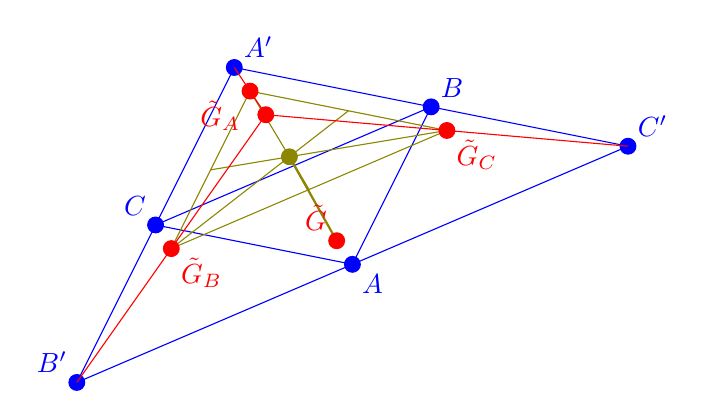
\begin{tikzpicture}[scale=2]
	\filldraw[blue] (0, 0) circle (0.05) node[above right] {$A'$};
	\filldraw[blue] (.75, -1.25) circle (0.05) node[below right] {$A$};
	\filldraw[blue] (-1, -2) circle (0.05) node[above left] {$B'$};
	\filldraw[blue] (1.25, -.25) circle (0.05) node[above right] {$B$};
	\filldraw[blue] (2.5, -.5) circle (0.05) node[above right] {$C'$};
	\filldraw[blue] (-.5, -1) circle (0.05) node[above left] {$C$};
	\draw[blue] (.75, -1.25) -- (1.25, -.25);
	\draw[blue] (1.25, -.25) -- (-.5, -1);
	\draw[blue] (-.5, -1) -- (.75, -1.25);

	\draw[blue] (0, 0) -- (-1, -2);
	\draw[blue] (-1, -2) -- (2.5, -.5);
	\draw[blue] (2.5, -.5) -- (0, 0);

	%\filldraw[red] (-.5, -1) circle (0.05) node[above left] {$M$};
	%\draw[red] (-.5, -1) -- (2.5, -.5);

	\draw[olive] (.1, -.15) -- (-.4, -1.15);
	\draw[olive] (-.4, -1.15) -- (1.35, -.4);
	\draw[olive] (1.35, -.4) -- (.1, -.15);

	\draw[olive] (.1, -.15) -- (0.475, -0.775);
	\draw[olive] (-.4, -1.15) -- (0.725, -0.275);
	\draw[olive] (1.35, -.4) -- (-.15, -.65);

	\filldraw[red] (.1, -.15) circle (0.05) node[below left] {$\tilde G_A$};
	\filldraw[red] (.2, -.3) circle (0.05);
	\filldraw[red] (-.4, -1.15) circle (0.05) node[below right] {$\tilde G_B$};
	\filldraw[red] (1.35, -.4) circle (0.05) node[below right] {$\tilde G_C$};

	\draw[thick, olive] (0.35, -0.567) -- (.65, -1.1);
	\filldraw[olive] (0.35, -0.567) circle (0.05);
	\filldraw[red] (.65, -1.1) circle (0.05) node[above left] {$\tilde G$};

	\draw[red] (0, 0) -- (.2, -.3);
	\draw[red] (-1, -2) -- (.2, -.3);
	\draw[red] (2.5, -.5) -- (.2, -.3);

\end{tikzpicture}\end{center}
$d$-wymiarowe uogólnienie trójkąta (jako otoczki wypukłej $d+1=3$ niewspółliniowych punktów) nazywamy $d$-sympleksem. Ogólniejsza wersja twierdzenia 1:
\\\textbf{Twierdzenie 1.1. Średnia wierzchołków (przy okazji wszystkich punktów) $d$-sympleksu leży na przecięciu odcinków łączących jego wierczhołki z barycentrami ścian naprzeciwko, i dzieli te odcinki w stosunku $1:d$.}
\\Dowód bo jest taki sam jak dla trójkątów.
\section{$f$-średnia}
Czasami trzeba uśrednić nie zmienną a coś co od niej zależy, np często używa się wartości napięcia ($U$) dla którego moc ($P=U^2/R$) będzie miała swoją średnią wartość (akurat tu nazywa się to wartością skuteczną napięcia). 
W tym wypadku uśredniamy (na przedziale długości $T$) kwadrat wartości funkcji $u(t)$, a potem bierzemy odpowiednią wartość $u$, tj\[
	U_s=\sqrt{\overline{u^2(t)}}=\sqrt{\frac1T\int_0^T(u(t))^2dt}
\]
i ogólnie oprócz kwadratowania można to robić z każdą inną funkcją (o ile jest odwracalna):\[
	\mu_f(a)=f^{-1}\Big(\overline{f(a)}\Big)
\]
\subsection{Nierówności między $f$-średnimi}
Na potrzeby tego pdf-u $\mu_f>\mu_g$ będzie oznaczać $\mu_f(a_1,a_2,\cdots,a_n) > \mu_g(a_1,a_2,\cdots,a_n)$ dla dowolnej ilości dowolnych danych.\\
\textbf{Twierdzenie 2. $\mu_f>\mu_g$ jeśli $f$ jest funkcją rosnącą a $g(f^{-1}(x))$ --- wypukłą
\\Dowód. }Niech:
\\\indent 1) danymi będą $a_1, \cdots, a_n$,
\\\indent 2) $\alpha_i=f^{-1}(a_i)$, 
\\\indent 3) $g(f^{-1}(x))=h(x)$ (oczywiście jest funkcją wypukłą).
\\Wtedy $f(\mu_f(\alpha_1,\cdots,\alpha_n))=\mu(a_1, \cdots, a_n)$, a $f(\mu_g(\alpha_1,\cdots,\alpha_n))=\mu_h(a_1, \cdots, a_n)$.
Rysujemy:
\\\indent 1) wykres funkcji $h$,
\\\indent 2) $n$ prostych, gdzie $i$-ta z nich ma równanie $x=a_i$,
\\\indent 3) punkty (w sensie kropki) $A_1, \cdots, A_n$ w przecięciach prostych z wykresem,
\\\indent 4) punkty $B_1, \cdots, B_n$ w przecięciach prostych z odcinkiem $A_1A_n$,
\\\indent 5) prostą o równaniu $x=\mu(a_1, \cdots, a_n)$ przecinającą odcinek w punkcie $M$.
\begin{center}
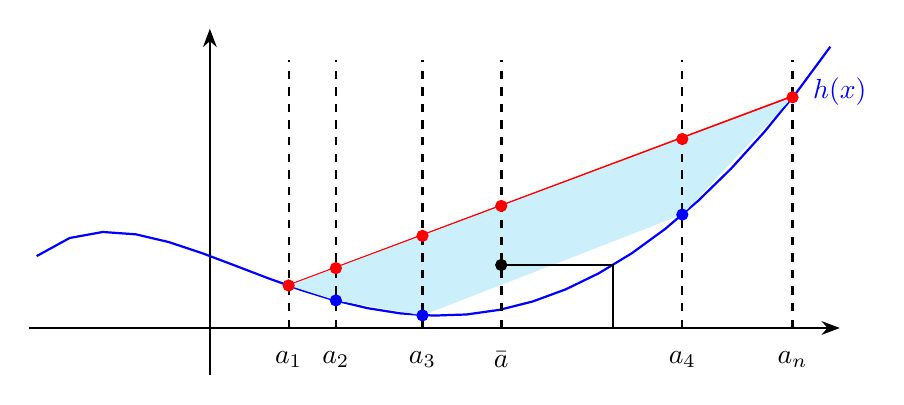
\begin{tikzpicture}
	\draw[-Stealth, thick] (-3.3, 0) -- (7, 0);
	\draw[-Stealth, thick] (-1, -.6) -- (-1, 3.8);
	\draw[blue, thick, domain=-2:4.3] plot (1.6*\x, {0.3-0.13*(exp(1.4-\x)-3*(\x-1.4)^2)});%*((\x-1.4)^2));
	\draw[red, thick, domain=0:4] plot (1.6*\x, 0.54+0.60*\x);

	\draw[blue] node at (7, 3) {$h(x)$};

	\fill[cyan!20] (0, 0.54) --(.6, 0.35) -- (1.7, 0.16) -- (5, 1.44) -- (6.4, 2.93);

	\draw node at (0, -.4) {$a_1$};
	\draw[thick, dashed] (0, 0) -- (0, 3.4);
	\filldraw[red] (0, 0.54) circle (2pt);

	\draw node at (.6, -.4) {$a_2$};
	\draw[thick, dashed] (.6, 0) -- (.6, 3.4);
	\filldraw[blue] (.6, 0.35) circle (2pt);
	\filldraw[red] (.6, 0.76) circle (2pt);

	\draw node at (1.7, -.4) {$a_3$};
	\draw[thick, dashed] (1.7, 0) -- (1.7, 3.4);
	\filldraw[blue] (1.7, 0.16) circle (2pt);
	\filldraw[red] (1.7, 1.17) circle (2pt);

	\draw node at (5, -.4) {$a_4$};
	\draw[thick, dashed] (5, 0) -- (5, 3.4);
	\filldraw[blue] (5, 1.44) circle (2pt);
	\filldraw[red] (5, 2.40) circle (2pt);

	\draw node at (6.4, -.4) {$a_n$};
	\draw[thick, dashed] (6.4, 0) -- (6.4, 3.4);
	\filldraw[red] (6.4, 2.93) circle (2pt);

	\draw node at (2.7, -.4) {$\bar a$};
	\draw[very thick, dashed] (2.7, 0) -- (2.7, 3.4);
	\filldraw[black] (2.7, 0.8) circle (2pt);
	\filldraw[red] (2.7, 1.55) circle (2pt);

	\draw (2.7, 0.8) -- (4.12, 0.8) -- (4.12, 0);
\end{tikzpicture}
\end{center}
Punkt $M$ jest śrenią punktów $B_1, \cdots, B_n$, bo leży na odcinku $B_1B_n$ i jego współrzędna $x$ się zgadza (jest tylko 1 taki punkt). 
Liczba $\mu_h(a_1, \cdots, a_n)$ to taka $x$ że $h(x)$ jest współrzędną $y$ średniej punktów $A_1, \cdots, A_n$.
Ta średnia leży pod punktem $M$ (bo ma tą samą współrzędną $x$ i leży w otoczce wypukłej punktów $A_1, \cdots, A_n$), 
a więc prosta pozioma przechodząca przez nią przecina wykres funkcji $h$ gdzieś po prawo, tj. dla większej wartości $x$ niż współrzędna $x$ punktu $M$.
A ponieważ ta pierwsza wynosi $f(\mu_g(\alpha_1,\cdots,\alpha_n))$ a druga --- $f(\mu_f(\alpha_1,\cdots,\alpha_n))$ (a $f$ jest rosnąca), to istotnie $\mu_f(\alpha_1,\cdots,\alpha_n)) > \mu_g(\alpha_1,\cdots,\alpha_n)$ $\square$\\
To samo zadziała jeśli $f$ będzie malejąca a $h$ --- wklęsła; za to oba warunki na raz można zapisać $f'\cdot(g\circ f^{-1})'>0$.
Jeśli $f$ i $g$ są ciągłe (zazwyczaj są) i odwracalne (muszą takie być żeby dało się robić $f$-średnią) to muszą być albo rosnące albo malejące w całej dziedzinie, a warunek $f'\cdot(g\circ f^{-1})'>0$ robi się (tak to się ładnie nazywa) konieczny i wystarczający.
\\Teraz kilka uszczególnień, na ich potrzeby będziemy używali takiego symbolu:
\\$\bullet$ $\mu_a:=\mu_{x^a}$ dla $a\neq 0$,
\\$\bullet$ $\mu_0:=\lim_{a\to0}\mu_a=\mu_{\ln(x)}=\sqrt[n]{a_1a_2\cdots a_n}$ (średnia geometryczna),
\\$\bullet$ $\mu_{+\infty}:=\lim_{a\to+\infty}\mu_a=\max{a_1, a_2, \cdots, a_n}$ (maksimum),
\\$\bullet$ $\mu_{-\infty}:=\lim_{a\to-\infty}\mu_a=\min{a_1, a_2, \cdots, a_n}$ (minimum).
\\\textbf{Twierdzenie 3. $\mu_a>\mu_b$ iff $a>b$
\\Dowód dla $b\neq 1$:
\\oczywiście funkcja $x^a$ jest rosnąca a funkcja $x^{a-b}$ jest wklęsła iff $a>b$ $\square$
\\Dowód dla $b=1$:
\\funkcja $e^{ax}$ jest wklęsła iff $a>0$ $\square$
\\Dowód dla $b=+\infty$:
\\niech ciąg $a_1, a_2, \cdots, a_n$ będzie nierosnący. Wtedy $\frac1{\sqrt{n}}\sqrt[a]{a_1, a_2\cdots, a_n} < \frac1{\sqrt[a]{n}}\sqrt[a]{a_1, a_1, \cdots, a_1} = a_1$ $\square$.
\\Dowód dla $b=-\infty$:
\\niech ciąg $a_1, a_2, \cdots, a_n$ będzie niemalejący. Wtedy $\frac1{\sqrt{n}}\sqrt[a]{a_1, a_2\cdots, a_n} > \frac1{\sqrt[a]{n}}\sqrt[a]{a_1, a_1, \cdots, a_1} = a_1$ $\square$.
}
Jeśli $a_1=a_2=\cdots=a_n$ to zamiast znaku $<$ mamy znak $=$ (uprzednio zakładaliśmy że dane nie są wszystkie takie same).
\\W szczególności:\[
	\mu_{x^2}>\mu_x>\mu_{\ln(x)}>\mu{\frac1x}
\]
innymi słowy\[K>A>G>H\]
\end{document}
% editing test cause it's not working for some reason
